%(BEGIN_QUESTION)
% Copyright 2007, Tony R. Kuphaldt, released under the Creative Commons Attribution License (v 1.0)
% This means you may do almost anything with this work of mine, so long as you give me proper credit

Her vises responsen til en prosess på en serie trinnendringer i regulatorutgangen (alle gjort mens regulatoren stod i ``manuell'' modus). Hva kan du, basert på observasjonene dine, fastslå om prosessen og tilhørende instrumentering?

$$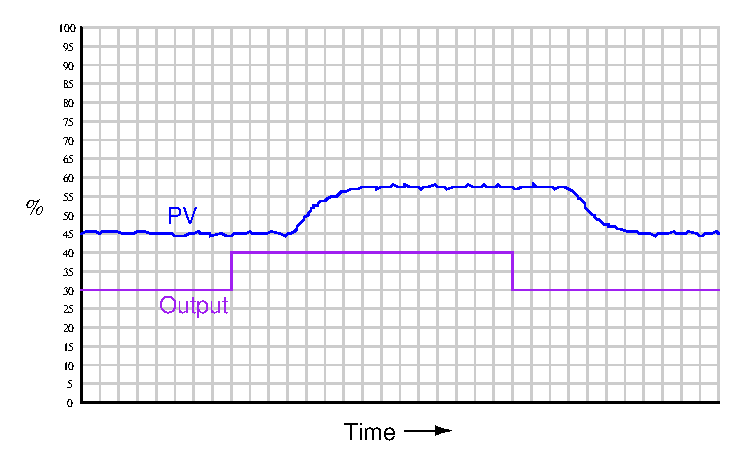
\includegraphics[width=15.5cm]{i01650x01.eps}$$

Beregn også den {\it stasjonære forsterkningen} ($K$) for denne prosessen, basert på trenden over.

\underbar{file i01650}
%(END_QUESTION)





%(BEGIN_ANSWER)

Dette plottet av PV-respons for flere trinnendringer i utgangen viser at prosessen har en betydelig mengde {\it dødtid}, teknisk kjent som {\it transportforsinkelse}. Det finnes mange mulige årsaker til dødtid, men den vanligste er dårlig plassering av primærsensorelementet (PSE), slik at det må gå en merkbar tid før prosessstrømmen fører resultatet av sluttregulerende element sin endring frem til sensoren. Et eksempel er temperaturregulering av emner på et transportbånd, der temperaturføler og varmeelement er plassert langt fra hverandre på båndet:

$$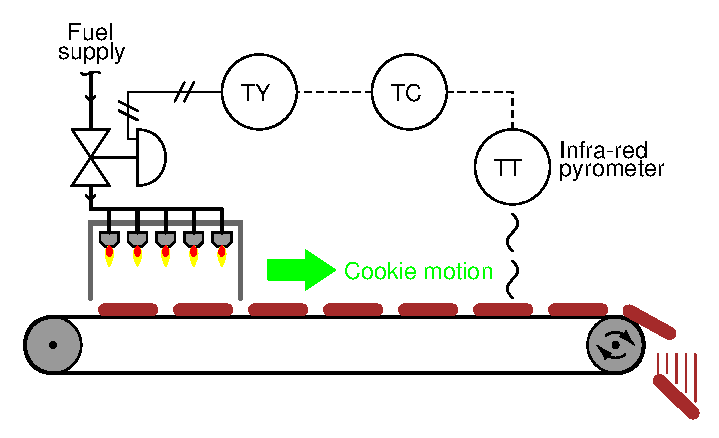
\includegraphics[width=15.5cm]{i01650x02.eps}$$

Det finnes likevel andre muligheter. Dette fenomenet kan for eksempel også skyldes en kombinasjon av stiction og begrenset luftstrøm i en pneumatisk ventilaktuator.

\vskip 10pt

Den {\it stasjonære forsterkningen} til en selvregulerende prosess er definert som endringen i prosessvariabel ($\Delta$PV) som følge av en endring i manipulert variabel ($\Delta$Output). I dette tilfellet ga en trinnendring på 10\% i utgangen omtrent 12.5\% endring i prosessvariabelen (fra omtrent 45\% til omtrent 57.5\%): et forholdstall på 1.25.

\vskip 10pt

$K$ = 1.25 (omtrent)

%(END_ANSWER)





%(BEGIN_NOTES)


%INDEX% Control, PID tuning: step change (output) revealing hysteresis

%(END_NOTES)
